% Number 380
% CAPM
% Skateboarder jump a direction determination
% JG

% Watermark
\AddToShipoutPicture*{\BackgroundPic}

\addtocounter {ProbNum} {1}

%\begin{floatingfigure}[r]{.15\textwidth}
%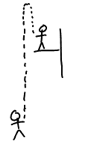
\includegraphics[scale=.8]{/Users/jgates/desktop/latex/pics/tokentoss.png}
%\end{floatingfigure}
 
{\bf \Large{\arabic{ProbNum}}} A diagram of a crazy skateboarder's stunt is shown below.  The skateboarder begins at rest at the top of the ramp, goes down the ramp, up the small ramp, and flies off of the ramp.  Do the following:


\MakeList{a.}{
\item Draw and label acceleration vectors for sections A, B, and C.  That�s three vectors to draw. 
\item Draw and label initial and final velocity vectors for sections A and B -- that's four more vectors to draw.  Place the tails of these vectors at the ends of the dotted segments denoting the three sections.  Make their lengths proportionate to the speeds. 
}

\begin{center}
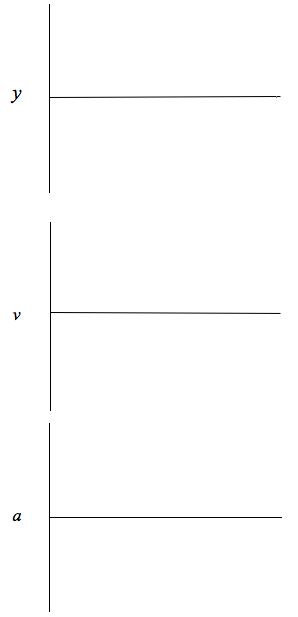
\includegraphics[scale=.85]{/Users/jgates/desktop/latex/pics/blankyvagraphstack.png}
\end{center}


\vfill
\newpage
